\chapter{Past Simple: Basic Past Tense}

\begin{center}
\begin{tabular}{ccc}
\cefrlevel{A1-A2} & \textbf{Study Time:} 2-3 hours & \textbf{Difficulty:} ⭐⭐☆☆☆
\end{tabular}
\end{center}

\section{Lesson Objectives}
In this chapter, you will learn:
\begin{itemize}
    \item How to form the Past Simple with regular and irregular verbs
    \item When to use Past Simple
    \item How to make negative sentences and questions
    \item Common time expressions with Past Simple
    \item The difference between regular and irregular verbs
\end{itemize}

\section{Reading Context}
\begin{readingbox}[title=Dialogue: Last Weekend]
\textbf{Sarah:} What did you get up to last weekend?\\
\textbf{Mike:} I \textbf{went} to the cinema on Saturday night. I \textbf{saw} the new James Bond film at the Odeon.\\
\textbf{Sarah:} Oh brilliant! \textbf{Did} you \textbf{enjoy} it?\\
\textbf{Mike:} Yes, I \textbf{loved} it! It \textbf{was} absolutely brilliant. The action scenes were ace! What about you?\\
\textbf{Sarah:} I \textbf{stayed} in, I'm afraid. I \textbf{didn't go} out because I \textbf{had} a dreadful cold and \textbf{felt} quite poorly.\\
\textbf{Mike:} Oh dear, that's rotten luck. \textbf{Did} you \textbf{manage} to rest?\\
\textbf{Sarah:} Yes. I \textbf{watched} telly and \textbf{read} a good book. I also \textbf{rang} my mum for a proper chat.\\
\textbf{Mike:} Good on you. Are you feeling better now?\\
\textbf{Sarah:} Yes, much better, cheers!
\end{readingbox}

\begin{britishbox}[title=🇬🇧 British Cinema and Entertainment Culture]
\textbf{Vocabulario esencial del cine británico:}
\begin{itemize}
    \item \textbf{Film} (NOT "movie") - "Did you see that film?"
    \item \textbf{Cinema} (NOT "theater") - "Let's go to the cinema"
    \item \textbf{Odeon, Vue, Cineworld} - Main British cinema chains
    \item \textbf{Screen} - Cinema room: "It's showing on screen 5"
\end{itemize}

\textbf{Typical British weekend activities:}
\begin{itemize}
    \item \textbf{Sunday roast} - Traditional Sunday meal (roast beef/chicken, Yorkshire pudding, roast potatoes, vegetables, gravy). Families gather at pubs or at home.
    \item \textbf{Going to the pub} - "We went to the local for a pint"
    \item \textbf{Watching football} - "I watched the match" (not "game")
    \item \textbf{Visiting National Trust properties} - Historic houses and gardens
\end{itemize}

\textbf{British expressions for being ill:}
\begin{itemize}
    \item "I felt \textbf{poorly}" (very British)
    \item "I was \textbf{under the weather}" (feeling unwell)
    \item "I had \textbf{a dreadful cold}" (a terrible cold)
    \item "I felt \textbf{quite rough}" (feeling awful)
\end{itemize}

\textbf{Fun fact:} James Bond (007) has been played by 7 actors, 6 of them British: Sean Connery (Scottish), Roger Moore, Timothy Dalton, Pierce Brosnan (Irish), Daniel Craig. He's the world's most famous British spy!
\end{britishbox}

\begin{comparisonbox}[title=🇪🇸 Pretérito vs Imperfecto: Una Trampa para Hispanohablantes]
\textbf{⚠️ PROBLEMA CLAVE:} En español tenemos DOS tiempos pasados (pretérito e imperfecto), pero en inglés Past Simple sirve para AMBOS.

\begin{center}
\begin{tabular}{|p{5.5cm}|p{5.5cm}|}
\hline
\textbf{Español (DOS formas)} & \textbf{Inglés (UNA forma)} \\
\hline
\textbf{Pretérito:} "Ayer \textit{jugué} fútbol" & \multirow{2}{*}{I \textbf{played} football} \\
\cline{1-1}
\textbf{Imperfecto:} "Cuando era niño \textit{jugaba} fútbol" & \\
\hline
\end{tabular}
\end{center}

\textbf{El contexto es clave:}
\begin{itemize}
    \item "I played football \textbf{yesterday}." → Pretérito (jugué)
    \item "When I was young, I played football." → Imperfecto (jugaba)
\end{itemize}

\textbf{💡 Para hábitos pasados, mejor usar:}
\begin{itemize}
    \item "I \textbf{used to} play football" (Solía jugar / Jugaba)
    \item "I \textbf{would} play football every Saturday" (Jugaba todos los sábados)
\end{itemize}
\end{comparisonbox}

\section{Grammar Focus: Past Simple Basics}

The Past Simple describes \textbf{completed actions in the past}.

\begin{grammarbox}[title=Past Simple - When to Use]
Use Past Simple for:
\begin{itemize}
    \item \textbf{Finished actions:} I \textbf{visited} Rome last year. \trans{Visité Roma...}
    \item \textbf{Past habits:} When I was young, I \textbf{played} football. \trans{Jugaba fútbol}
    \item \textbf{Series of past events:} I \textbf{woke up}, \textbf{had} breakfast, and \textbf{went} to work.
\end{itemize}
\end{grammarbox}

\section{Regular Verbs: Add -ED}

Most verbs are \textbf{regular}. To form the past, add \textbf{-ed}.

\begin{grammarbox}[title=Regular Verbs Structure]
\textbf{Affirmative:} Subject + \textbf{verb + ed}

\textbf{Examples:}
\begin{itemize}
    \item I \textbf{worked} yesterday. \trans{Trabajé ayer}
    \item She \textbf{played} tennis. \trans{Ella jugó tenis}
    \item They \textbf{watched} TV. \trans{Miraron TV}
\end{itemize}
\end{grammarbox}

\subsection{Spelling Rules for -ED}

\begin{table}[h]
\centering
\begin{tabular}{|l|l|l|}
\hline
\textbf{Rule} & \textbf{Example} & \textbf{Past Form} \\
\hline
Most verbs: add -ed & work, play, clean & worked, played, cleaned \\
\hline
Ends in -e: add -d only & live, like, move & lived, liked, moved \\
\hline
Ends in consonant + y: -ied & study, try, carry & studied, tried, carried \\
\hline
Ends in vowel + y: add -ed & play, enjoy, stay & played, enjoyed, stayed \\
\hline
One syllable CVC: double + ed & stop, plan, drop & stopped, planned, dropped \\
\hline
\end{tabular}
\caption{Spelling rules for regular past tense}
\end{table}

\subsection{Pronunciation of -ED}

\begin{table}[h]
\centering
\begin{tabular}{|l|l|l|}
\hline
\textbf{Sound} & \textbf{After these sounds} & \textbf{Examples} \\
\hline
/t/ & voiceless: k, p, f, s, sh, ch & worked, stopped, laughed, washed \\
\hline
/d/ & voiced: b, g, l, m, n, r, v, z & played, lived, cleaned, opened \\
\hline
/id/ & after t or d & wanted, needed, decided, waited \\
\hline
\end{tabular}
\caption{Pronunciation of -ed endings}
\end{table}

\begin{pronunciationbox}[title=🔊 Pronunciation Tip for Spanish Speakers]
\textbf{Common Challenge:} Spanish speakers often add an extra syllable to -ed endings.

\begin{itemize}
    \item ❌ WRONG: "play-ed" (2 syllables) → Only with words ending in t/d!
    \item ✅ CORRECT: "played" /pleɪd/ (1 syllable) - like "pleid"
\end{itemize}

\textbf{Practice these:}
\begin{itemize}
    \item worked → /wɜːkt/ (one sound: "werkt")
    \item called → /kɔːld/ (one sound: "cold")
    \item started → /ˈstɑːtɪd/ (two syllables: "star-tid") ← Only this type gets extra syllable!
\end{itemize}

\textbf{Memory trick:} If the verb already ends in T or D sound, add /ɪd/. Otherwise, just add /t/ or /d/ sound!
\end{pronunciationbox}

\section{Irregular Verbs}

Many common verbs are \textbf{irregular}. They don't add -ed. You must learn them!

\begin{vocabbox}[title=Common Irregular Verbs]
\centering
\begin{tabular}{|l|l|l||l|l|l|}
\hline
\textbf{Infinitive} & \textbf{Past} & \textbf{Spanish} & \textbf{Infinitive} & \textbf{Past} & \textbf{Spanish} \\
\hline
be & was/were & ser/estar & have & had & tener \\
\hline
go & went & ir & do & did & hacer \\
\hline
come & came & venir & see & saw & ver \\
\hline
take & took & tomar & give & gave & dar \\
\hline
make & made & hacer & get & got & obtener \\
\hline
eat & ate & comer & drink & drank & beber \\
\hline
buy & bought & comprar & think & thought & pensar \\
\hline
write & wrote & escribir & read & read /red/ & leer \\
\hline
say & said & decir & tell & told & decir \\
\hline
know & knew & saber & meet & met & conocer \\
\hline
\end{tabular}
\end{vocabbox}

\begin{warningbox}[title=⚠️ IRREGULAR CONFUSO: READ]
\textbf{El verbo más confuso del inglés:}

\begin{center}
\begin{tabular}{|l|l|l|}
\hline
\textbf{Forma} & \textbf{Escritura} & \textbf{Pronunciación} \\
\hline
Present & read & /riːd/ ("riid") \\
\hline
Past & read & /red/ (como el color "red") \\
\hline
\end{tabular}
\end{center}

\textbf{Ejemplos:}
\begin{itemize}
    \item Present: "I \textbf{read} books every day" /riːd/
    \item Past: "Yesterday I \textbf{read} a book" /red/
\end{itemize}

\textbf{💡 Cómo distinguirlos:} Mira el contexto - palabras como "yesterday", "last week" indican pasado /red/
\end{warningbox}

\section{Negative Sentences}

\begin{grammarbox}[title=Past Simple Negative]
\textbf{Structure:} Subject + \textbf{didn't} + \textbf{base verb}

\textbf{Important:} The main verb stays in the BASE FORM (no -ed)!

\textbf{Examples:}
\begin{itemize}
    \item I \textbf{didn't work} yesterday. \trans{No trabajé ayer}
    \item She \textbf{didn't go} to the party. \trans{Ella no fue a la fiesta}
    \item They \textbf{didn't see} the movie. \trans{No vieron la película}
\end{itemize}

\textbf{Common Error:}
\begin{itemize}
    \item \textcolor{red}{I didn't worked.} \textbf{X} (WRONG)
    \item \textcolor{green!60!black}{I didn't work.} \checkmark (CORRECT)
\end{itemize}
\end{grammarbox}

\section{Questions}

\begin{grammarbox}[title=Past Simple Questions]
\textbf{Structure:} \textbf{Did} + subject + \textbf{base verb}?

\textbf{Examples:}
\begin{itemize}
    \item \textbf{Did} you \textbf{work} yesterday? \trans{¿Trabajaste ayer?}
    \item \textbf{Did} she \textbf{go} to London? \trans{¿Fue ella a Londres?}
    \item What \textbf{did} you \textbf{do}? \trans{¿Qué hiciste?}
\end{itemize}

\textbf{Short Answers:}
\begin{itemize}
    \item Yes, I did. / No, I didn't.
    \item Yes, she did. / No, she didn't.
\end{itemize}

\textbf{Exception - Verb TO BE:}
\begin{itemize}
    \item \textbf{Was} he at home? (NOT: Did he be...?)
    \item \textbf{Were} they happy? (NOT: Did they be...?)
\end{itemize}
\end{grammarbox}

\section{Time Expressions}

\begin{vocabbox}[title=Common Past Time Expressions]
\begin{itemize}
    \item \textbf{yesterday} \trans{ayer}
    \item \textbf{last} night/week/month/year \trans{anoche/la semana pasada...}
    \item \textbf{ago:} 2 days ago, 3 weeks ago \trans{hace 2 días, hace 3 semanas}
    \item \textbf{in:} in 2020, in July \trans{en 2020, en julio}
    \item \textbf{when I was} young/a child \trans{cuando era joven/niño}
    \item \textbf{this morning} (if morning is finished) \trans{esta mañana}
\end{itemize}
\end{vocabbox}

\subsection{Visual Guide: Past Simple Timeline}

\begin{center}
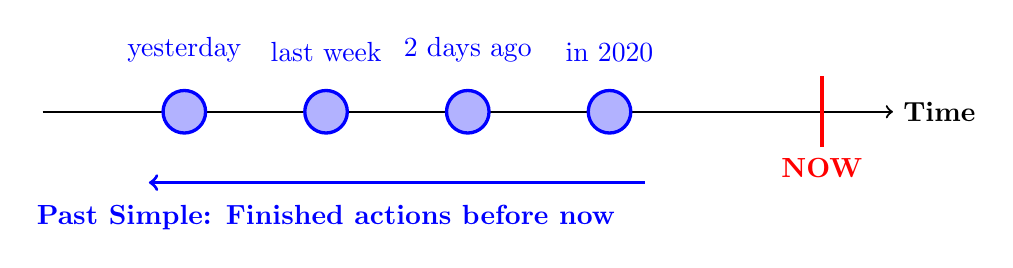
\begin{tikzpicture}[scale=0.9]
  % Timeline
  \draw[->, thick] (0,0) -- (12,0) node[right] {\textbf{Time}};
  
  % Past events
  \draw[blue, very thick, fill=blue!30] (2,0) circle (0.3) node[above=0.5cm] {yesterday};
  \draw[blue, very thick, fill=blue!30] (4,0) circle (0.3) node[above=0.5cm] {last week};
  \draw[blue, very thick, fill=blue!30] (6,0) circle (0.3) node[above=0.5cm] {2 days ago};
  \draw[blue, very thick, fill=blue!30] (8,0) circle (0.3) node[above=0.5cm] {in 2020};
  
  % "Now" marker
  \draw[red, very thick] (11,-0.5) -- (11,0.5);
  \node[red] at (11,-0.8) {\textbf{NOW}};
  
  % Past label
  \node[blue] at (4,-1.5) {\textbf{Past Simple: Finished actions before now}};
  
  % Arrow showing past
  \draw[blue, very thick, <-] (1.5,-1) -- (8.5,-1);
\end{tikzpicture}
\end{center}

\begin{notebox}[title=💡 Key Rule]
Use Past Simple for actions that are \textbf{FINISHED} and \textbf{COMPLETE}.
\begin{itemize}
    \item The time is specified or understood: \textit{I went to London \textbf{last year}.}
    \item The action is not connected to now: \textit{Shakespeare \textbf{wrote} many plays.}
\end{itemize}
\textbf{Important:} If you mention WHEN something happened, use Past Simple!
\end{notebox}

\section{Practice Exercises}

\subsection{Exercise 1: Write the Past Form}
Write the past simple form of these verbs.

\begin{table}[h]
\centering
\begin{tabular}{|l|l||l|l|}
\hline
\textbf{Infinitive} & \textbf{Past} & \textbf{Infinitive} & \textbf{Past} \\
\hline
work & \underline{\hspace{3cm}} & go & \underline{\hspace{3cm}} \\
\hline
study & \underline{\hspace{3cm}} & see & \underline{\hspace{3cm}} \\
\hline
stop & \underline{\hspace{3cm}} & have & \underline{\hspace{3cm}} \\
\hline
play & \underline{\hspace{3cm}} & make & \underline{\hspace{3cm}} \\
\hline
live & \underline{\hspace{3cm}} & eat & \underline{\hspace{3cm}} \\
\hline
\end{tabular}
\end{table}

\subsection{Exercise 2: Complete the Sentences}
Fill in the blanks with the past simple form.

\begin{enumerate}
    \item I \underline{\hspace{3cm}} (visit) my grandparents last weekend.
    \item She \underline{\hspace{3cm}} (not/go) to work yesterday.
    \item They \underline{\hspace{3cm}} (watch) a movie on Saturday.
    \item \underline{\hspace{3cm}} you \underline{\hspace{3cm}} (have) a good time?
    \item He \underline{\hspace{3cm}} (be) very tired last night.
    \item We \underline{\hspace{3cm}} (not/see) Tom at the party.
    \item What time \underline{\hspace{3cm}} she \underline{\hspace{3cm}} (arrive)?
\end{enumerate}

\subsection{Exercise 3: Make Questions}
Transform these sentences into questions.

\begin{enumerate}
    \item You went to the cinema. $\rightarrow$ \underline{\hspace{6cm}}
    \item She bought a new car. $\rightarrow$ \underline{\hspace{6cm}}
    \item They lived in Paris. $\rightarrow$ \underline{\hspace{6cm}}
    \item He ate pizza for dinner. $\rightarrow$ \underline{\hspace{6cm}}
\end{enumerate}

\subsection{Exercise 4: Correct the Errors}
Find and correct the mistakes in these sentences.

\begin{enumerate}
    \item I didn't went to school yesterday.
    \item Did she came to the meeting?
    \item He didn't bought the book.
    \item They goed to London last year.
    \item Did you saw the movie?
\end{enumerate}

\subsection{Exercise 5: Complete the Story}
Fill in the blanks with the correct past simple form.

Last Saturday, I \underline{\hspace{2cm}} (wake) up early. I \underline{\hspace{2cm}} (have) breakfast and then I \underline{\hspace{2cm}} (go) to the gym. I \underline{\hspace{2cm}} (exercise) for an hour. After that, I \underline{\hspace{2cm}} (meet) my friends for lunch. We \underline{\hspace{2cm}} (eat) at a nice restaurant. In the afternoon, we \underline{\hspace{2cm}} (watch) a football match. My team \underline{\hspace{2cm}} (win)! In the evening, I \underline{\hspace{2cm}} (be) very tired, so I \underline{\hspace{2cm}} (stay) home and \underline{\hspace{2cm}} (read) a book.

\subsection{Exercise 6: Writing Task}
Write a paragraph (80-100 words) about what you did last weekend. Use at least 8 verbs in the past simple.

\begin{tcolorbox}[colback=white,height=7cm]
% Write about your last weekend...
\end{tcolorbox}

\subsection{Exercise 7: British History Practice}
Complete these sentences about British history using the Past Simple.

\begin{enumerate}
    \item William Shakespeare \underline{\hspace{3cm}} (write) Romeo and Juliet in 1597.
    \item The Beatles \underline{\hspace{3cm}} (become) famous in the 1960s.
    \item Queen Victoria \underline{\hspace{3cm}} (rule) the British Empire for 63 years.
    \item Charles Dickens \underline{\hspace{3cm}} (create) many famous characters.
    \item The Tower of London \underline{\hspace{3cm}} (be) built nearly 1,000 years ago.
\end{enumerate}

\begin{britishbox}[title=🇬🇧 Famous British Historical Figures]
\textbf{Practice talking about these important Britons:}
\begin{itemize}
    \item \textbf{William Shakespeare} (1564-1616) - wrote famous plays like Hamlet and Macbeth
    \item \textbf{Queen Elizabeth I} (1533-1603) - ruled during the Golden Age
    \item \textbf{Isaac Newton} (1643-1727) - discovered gravity and laws of motion
    \item \textbf{Charles Darwin} (1809-1882) - developed the theory of evolution
    \item \textbf{Winston Churchill} (1874-1965) - led Britain during World War II
\end{itemize}
\textbf{Try this:} Write 5 sentences about one of these historical figures using Past Simple!
\end{britishbox}

\section{Key Takeaways}
\begin{itemize}
    \item \textbf{Regular verbs} add -ed in the past (worked, played)
    \item \textbf{Irregular verbs} change form (go $\rightarrow$ went, see $\rightarrow$ saw)
    \item In \textbf{negatives and questions}, use \textbf{didn't/did} + base verb
    \item The main verb stays in BASE FORM after did/didn't
    \item Learn irregular verbs - they're very common!
    \item Use time expressions: yesterday, last week, ago
\end{itemize}
